\documentclass[12pt]{article}

\usepackage[margin=1in]{geometry}
\usepackage{graphicx}
\usepackage{tocloft}
\renewcommand{\cftsecleader}{\cftdotfill{\cftdotsep}}
\renewcommand{\cftsecfont}{\bfseries\normalsize}
\usepackage[utf8]{inputenc}
\usepackage{placeins}
\usepackage{amsmath}
\usepackage{titlesec}
\usepackage{float}
\usepackage{booktabs}% http://ctan.org/pkg/booktabs
\newcommand{\tabitem}{~~\llap{\textbullet}~~}
\usepackage{tabularx}

\begin{document}
	\title{BottleGuard\\Final Report}
	\author{Duy Duong\\UID: 505183737 \and Alex Best \and Nayiree Dahyet \and Samritha Nagesh \and Jesus Martin \and Joshia Iglesia \and Timothy Yu}
	\date{\today}
	\maketitle

	
	\section*{Proposal support}
	\begin{center}
			Name \underline{\hspace{8cm}}
		Signature \underline{\hspace{3cm}}\\ \vspace{5mm}
		Name \underline{\hspace{8cm}}
		Signature \underline{\hspace{3cm}}\\  \vspace{5mm}
		Name \underline{\hspace{8cm}}
		Signature \underline{\hspace{3cm}}\\  \vspace{5mm}
		Name \underline{\hspace{8cm}}
		Signature \underline{\hspace{3cm}}\\  \vspace{5mm}
		Name \underline{\hspace{8cm}}
		Signature \underline{\hspace{3cm}}\\  \vspace{5mm}
		Name \underline{\hspace{8cm}}
		Signature \underline{\hspace{3cm}}\\  \vspace{5mm}
		Name \underline{\hspace{8cm}}
		Signature \underline{\hspace{3cm}}\\  \vspace{5mm}
	\end{center}

\pagebreak
	\renewcommand*\contentsname{Table of Contents}
	\tableofcontents
		\vspace{10mm}
		
	\setlength{\parindent}{4em}
	\setlength{\parskip}{1em}
		\pagebreak
	\addcontentsline{toc}{section}{Abstract}
	\begin{abstract}
		While inhabiting shared living spaces like apartments have their advantages, such as cheaper living, they also have their fair share of annoyances, one of which being sharing beverage items.  Often times, it becomes hard  to effectively convey one’s preferences for what items should be shared and to what extent the sharing of that item should continue.  Additionally, it is hard to mitigate other individuals from simply disregarding another’s sharing preferences, and over indulging in their generosity.  The BottleGuard can assuage these problems by allowing the owner to communicate in real time to their apartment mates whether they want to share or not from anywhere in the world.  With a complimentary app, BottleGuard can be controlled remotely from anywhere with internet, signalling the owner’s sharing preference via a multi-colored led.  Users will also be notified of unwelcome use of their beverages as BottleGuard replaces the bottle’s original cap, and notifies owners of use with a gyroscope sensor built into the cap.  At a rather competitive price of \$25, 13,107 units will need to be sold in order to break even on the production and development costs.  Through proper production scheduling and adequate risk prevention and mitigation, BottleGuard will soon bring to customers the ability to share when desired while also maintaining the peace of mind that they won’t be taken advantage of.
	\end{abstract}

		\addcontentsline{toc}{section}{Introduction}
	\section*{Introduction}
	\hspace{4em}Bailey is a college student who lives in an apartment with several roommates. They all share the same fridge, and some of the items within. Although she is generally fine sharing her drinks with others, sometimes Bailey would like to keep them to herself when she gets a soda that is difficult to find or when the drink is running out. Due to their busy schedules, however, she finds it difficult to communicate that with all of her roommates. She resents the fact that sometimes her roommates help themselves to her drinks without asking for permission first because they were not aware that she didn't want to share. Bailey would like a way to remind her roommates in the moment of whether or not she is willing to share. Additionally, she wants to know when someone tries to open the bottle and take her soda when she has not granted permission.
	
	She has tried different methods of expressing her intentions, such as sticking Post-it notes on her bottles or sending a text message to their roommate group that she'd prefer if they didn't take her drink. However, these methods have not proven to be effective since text messages are often ignored or overlooked, and Post-it notes are prone to falling off the bottle. She finds a bottle lock called KwikTop but decides against using it since she understands that everyone’s schedule is different from hers, and such an inflexible method of keeping the drink to herself defeats the idea of sharing the drink, and can sour Bailey’s relationship with her roommates. Moreover, a bottle lock comes at a fixed size and can only fit on one type of bottle, while she wishes to share a variety of drinks that come in markedly different bottle sizes like soda bottles or milk jugs. IIdeally, she also wants something that does not take up much room in the fridge, as she only has a limited amount of fridge space allocated to her.
	
	Our device, BottleGuard, will solve all of Bailey’s problems, providing an advantage over competitors by allowing for a nearly instantaneous response notification to attempted use and to communicate the owner’s preferences to all users. BottleGuard is a compact cap replacement that can be fitted on to various types of bottles. It would let Bailey’s roommates know if she wanted to share the drink through a sharing mode that displays a green light to indicate a desire to share and a red light to indicate when one does not want to share. With a simple button press from the app, Bailey can set the light on the device from red to green from anywhere in the world with an Internet connection. The green light would then indicate her consent to share for the next couple minutes, allowing her roommate to pour their drink, before changing back to red again and signifying that permission is needed.  Bailey can also choose to keep the light green and leave sharing open. When the light is red, any attempt to open the bottle will trigger a warning sound and send a notification with the time the bottle was opened to Bailey’s phone. Bailey can now be more secure in knowing that she can be aware of if and when her roommates try to take her drinks, or use them without permission.
	
	There are a few risks inherent with BottleGuard, but nothing too dire.  The largest risks come from users trying to misuse the device by subjecting it to environments that BottleGuard was not designed for such as an oven or microwave.  These risks will be covered with more depth later on, however the greatest mitigation factor for a majority of the risks will be found in warning and instructions provided in a manual with each device.  BottleGuard is priced at a competitive twenty five dollars per device, allowing for the company to break even after the sale of approximately 13,107 units.  
	
		\addcontentsline{toc}{section}{Market overview: Price / Performance}
	\section*{Market overview: Price / Performance}
		\addcontentsline{toc}{subsection}{Price Performance Chart and Key Attribute Matrix}
	\subsection*{Price Performance Chart and Key Attribute Matrix}
	\begin{figure}[H]
		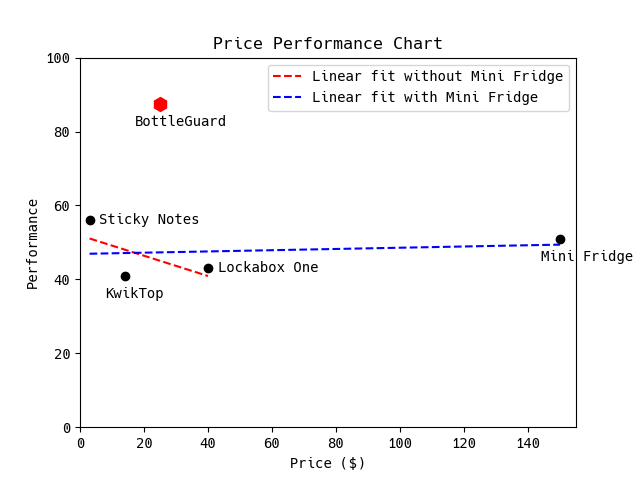
\includegraphics[width=\textwidth]{e185ew.png}
		\label{fig:ppc}
		\caption{Price Performance Chart}
	\end{figure}
\begin{figure}[H]
	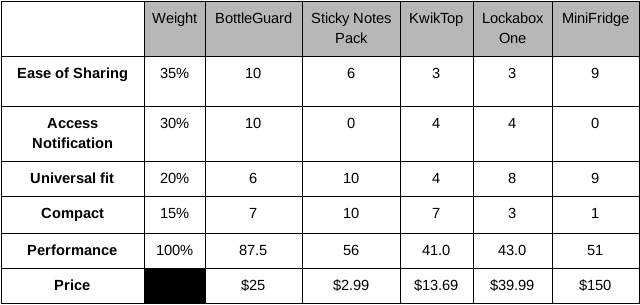
\includegraphics[width=\textwidth]{kam.png}
	\label{fig:kam}
	\caption{Key Attribute Matrix}
\end{figure}
	\addcontentsline{toc}{subsection}{Competition}
	\subsection*{Competition}
	The top competitors for Bottleguard are Kwiktop and a pack of sticky notes. Kwiktop is a combination lock that prevents access to the beverage without the combination. This product does not allow the user to easily share the beverage because the user is locking the bottle and nobody except the user could drink. If the user does not lock the bottle, other person may assume that can take the beverage without knowing that the user did not want to share. The sticky notes are cheap and can be used in every bottle. However, this solution does not allow the user to share or not share without physical intervention. If the user had a no sharing note but now wants to share, the user has to change the note, which sometimes will be complicated because the user is not in that place at that time. Also, the notes will not notify the user when someone is taking the beverage.
	
	The competitive advantage that Bottleguard has over its competitors is the ability to express willing to share or not share the beverage. With the app, the user only needs to press one button to tell others that they can drink the beverage, or that they are not allowed to drink. This ability that the user has, added to a notification every time someone is opening the bottle and a price that is not as high as the price of other products gives Bottleguard a good place in the Price Performance chart, above the linear fit. The linear fit is decreasing since the performance of the sticky notes is better than the performance of the rest of the competitors, and the price is lower. 
	
		\addcontentsline{toc}{subsection}{Key Attributes}
	\subsection*{Key Attributes}
	The unmet need story highlights the ability to share the beverage whenever the user wants to without being physically present, therefore ease of sharing is the most important key attribute. Without this attribute, the user is unable to express willing to share or not share the beverage. If the user is willing to share but did not tell anyone, a person who wants to take the beverage will have to ask for permission first or will not take the drink assuming no permission, which could be inconvenient for the user. But if the user do not want to share and did not notify others, they could take the beverage assuming permission is given. Next, the access notification is an important attribute to look for in the product because without access notification the user would not know when someone is taking beverage without permission. Following access notification comes universal fit. This attribute allows the user to use the product in a variety of bottles with different cap sizes, which allows the user to enjoy different beverages without having to buy different products for different bottles. Finally, compactness allows the user to use the product without taking too much space in the fridge or any place where the user keeps the bottle.
	
		\addcontentsline{toc}{subsection}{Price}
	\subsection*{Price}
	All products are a one time purchase except for the sticky notes pack, which has to be bought when the pack is finished. Since Bottlecap battery is rechargeable, there is no need to buy extra batteries or replacements for the device. Also, the competitors  do not require parts replacement. This means that the price is the total amount that the user will have to spend to use the products. 
	
			\addcontentsline{toc}{section}{Product Overview}
	\section*{Product Overview}

	\addcontentsline{toc}{section}{Program Risk and Mitigation}
	\section*{Program Risk and Mitigation}
	In terms of consumer reception risk, there is a possibility that consumers will opt for the cheaper sticky notes or KwikTop instead. To mitigate this risk, we will market BottleGuard’s ease of sharing and ability to notify, which are attributes that are uncharacteristic of other products in its price vicinity. Other than that, we believe our asking price of \$25 should not significantly deter consumers from purchasing the product for any other reasons.
	
	In terms of failure modes, one possible complication is the development of mold or other bacteria on the device as a result of the user failing to properly wash it. To illustrate, the mold could come in contact with the bottle contents. When the user drinks the bottle contents, he/she becomes unknowingly poisoned. This can lead to severe upset stomachs and nausea/vomiting. To mitigate the risk of this scenario occurring, we will add a clear warning in the instruction manual stating that the device needs to be regularly washed to avoid this issue. 
	
	A second possible complication is that the small size of the device makes it a choking hazard. This primarily applies to young children, who may easily access the device, attempt to eat it, and choke. This could have fatal consequences. In order to mitigate this risk, we will add a choking hazard warning label, a warning directed at parents that detail it is unsafe to leave unsupervised children with the device, and an age restriction to further deter unsupervised children from playing with device.
	
	Lastly, a possible complication may arise from heating the device to sufficiently high temperatures. Our device is not engineered to withstand high heat sources such as microwaves and ovens. In these cases, heated batteries may pose serious harm if they release flammable substances and are ignited, creating an explosion. To mitigate this risk, we will include a warning label that directs users to not use the device in microwaves, ovens, or any other areas with high heat.
	
	
	
	
		\addcontentsline{toc}{section}{Financial Summary}
	\section*{Financial Summary}
		\addcontentsline{toc}{subsection}{Key Milestones}
	\subsection*{Key Milestones}
	\begin{itemize}
		\item 	Unit cost: \$4.069
		\item Unit retail price: \$25
		\item Development cost: \$274.4K
		\item Break even quantity: 13107
	\end{itemize}

	
	\addcontentsline{toc}{subsection}{Unit Cost Breakdown}
	\subsection*{Unit Cost Breakdown}
		\begin{figure}[H]
		\centering
		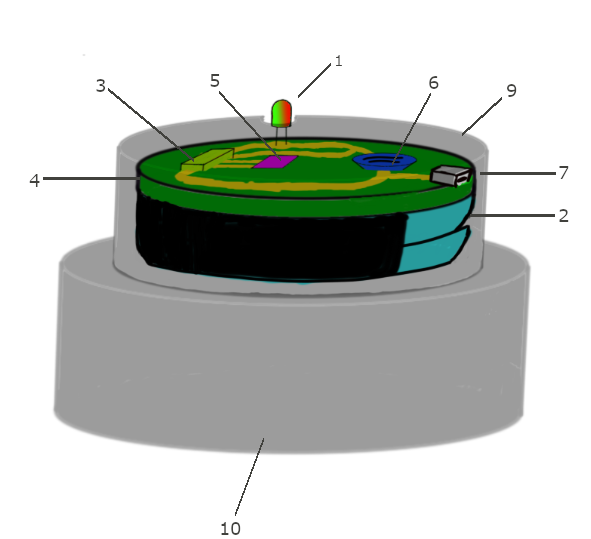
\includegraphics[width=10cm ]{DesignLabeled.png}
		\label{fig:design}
		\caption{Side view of BottleGuard with all parts labeled with their ID from the BOM below.}
	\end{figure}
\begin{table}[H]
	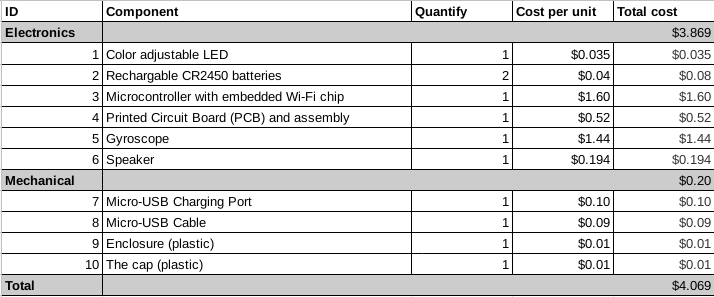
\includegraphics[width=\textwidth]{bom_small.png}
	\label{fig:bom}
	\caption{Detailed Bill of Materials for each part in BottleGuard. BOM with MOQ and part numbers/links to source vendors is included in the appendix..}
\end{table}
	\addcontentsline{toc}{subsection}{Development Cost Breakdown}
	\subsection*{Development Cost Breakdown}
	\subsubsection*{Labor: \$258K}
		\begin{table}[H]
		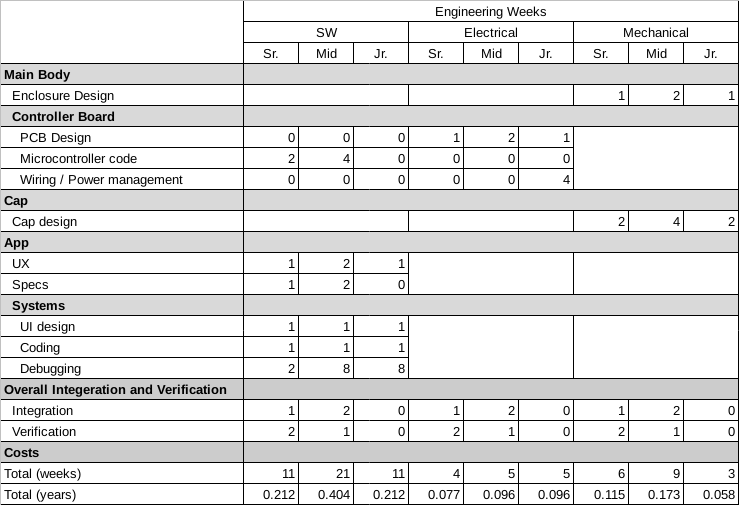
\includegraphics[width=\textwidth]{wbs_small.png}

		\caption{Estimated work weeks required for the development of BottleGuard. Detailed WBS with salary calculations as well as manager / benefits calculations is included in the appendix.}
	\end{table}
From the work weeks in Table 2 and standard industry salaries, the total salary needed for engineers is \$127K. With department managers and project managers each needing 25\% of total engineering time, we would need an additional \$44K for department managers and \$35.3K for project manager. In total, it would take \$206.4K for all labor costs, which comes up to \$258K with 25\% benefits.
	\subsubsection*{Capital: \$5K}
Since BottleGuard’s outer design is relatively simple, molds and tooling for the enclosure and the cap would cost an estimated \$5K total.
	\subsubsection*{NRE: \$10K}
	The universal cap design is the most important part of the design, and thus an extra \$10K is allocated to the mechanical engineers to help expedite the process. This money will go towards buying required equipment for testing as well as contracting any external help if needed.
	
	\subsubsection*{Risk Inventory: \$2.7K}
	As BottleGuard’s break even quantity (13107) is way above the MOQ of almost all components, we can keep a low risk inventory on all of them. One notable exception is the gyroscope, which must be purchased in reels of 5000. With the break even quantity of 13107, we would have to order 15000 gyroscopes at \$1.44, leaving us with 1893 gyroscopes as risk inventory. The total cost for this risk inventory is \$2.7K. 
	
	\addcontentsline{toc}{subsection}{Break Even Quantity Analysis}
	\subsection*{Break Even Quantity Analysis}
	Each unit is being sold for a retail price of \$25 for a profit of \$21 per device. The total development cost including labor, capital, NRE, and risk inventory is \$274.4K, giving us:
	\[ \text{Break Even Quantity} = \frac{\text{Total Development Cost}}{\text{Profit per unit}} = 13107 \] 
	The complete calculation including the initial break even calculation as well as the first pass to reduce MOQ is included in the appendix.
	
		\addcontentsline{toc}{section}{Delivery Date and Key Milestones}
	\section*{Delivery Date and Key Milestones}
Our three engineering teams (Software, Electrical, and Mechanical) will work towards completing our main deliverables, which are the app, electronics, plastic cap, and the final product after integration and verification. The chart below shows the complete breakdown of the weeks needed per deliverable as well as what each team is responsible for. The software team will be working on the app, which we estimate to take 5 weeks. The plastic cap will be completed by the mechanical engineering team at the end of 6 weeks. The electrical engineering will design and wire the electronic components, while the software team will code the microcontroller. The electronic components for the device will be ready by the end of week 8. After 4 weeks of integration and verification by all teams, the prototype will be completed. We estimate the full product design to take around 16 weeks, and during this time period we will continually improve our design and try to make the cycle more efficient. Accounting for the time needed to set up mass production, marketing, and some other operations, we expect our product to enter the market within a year. 
\begin{figure}[H]
	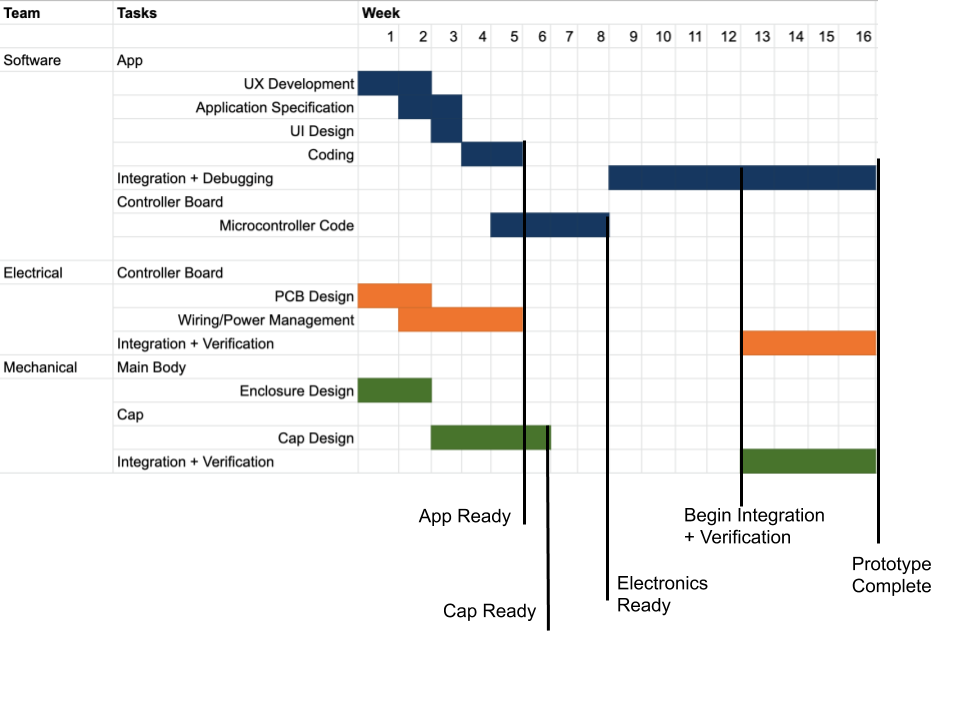
\includegraphics[width=\textwidth]{milestones.png}
	\label{fig:milestones}
	\caption{Complete product development cycle with key milestones marked}
\end{figure}
	\addcontentsline{toc}{section}{Summary and Recommendations}
	\section*{Summary and Recommendations}
		
		Nowadays, most young adults share their living spaces with roommates, or friends and this includes sharing the refrigerator. Some of them, like the case with our customer Bailey, want to share their beverages. However, they also like to control the sharing process including the times they want to share and the times they don’t. As illustrated in the previous sections, Bottle-Guard is the best fit. 
		
		Bottle-Guard stands strong among other competitors through helping the customers in the process of sharing of their drinks by showing to others the customers intention of sharing or not. That will happen through a simple APP that controls the red or green light shown on top of the device without the need of the physical attendance of the customer. Most importantly, it gives the customer the flexibility, by just a simple touch of a button using an APP on the phone, to give permission to share the drinks. Moreover, Bottle-Guard will simply send notification through an APP to the customer when someone tries to open the cap without asking for permission (or when the bottle is on the “not sharing” mode). Plus the alarms will go on when someone opens the bottle without permission. It is important to mention that our device is perfectly designed with its smart sensor to not give false notification if someone just moves the bottle or relocates it in the fridge. In addition, as illustrated in the previous sections, our product fits most standard caps and it is compact, does not take much space in the fridge. 
		
		Studies show that almost 79 million U.S. adults are living in shared household. Which increases our buyers market. Moreover, our device will help people not only in their houses, but also in their working place where they share the refrigerator with coworkers which will the increasing number of targeted customers. With that being said, plus our financial analysis, we believe that Bottle-Guard will succeed in the marketplace financially. Bottle-Guard will be the new product that will help customers share their drinks and control the process of sharing.
		
		\newpage
		\addcontentsline{toc}{section}{Appendix}
		\section*{Appendix}
			\addcontentsline{toc}{subsection}{Unmet Need}
		\subsection*{Unmet Need}
		Bailey is a college student who lives in an apartment with several roommates. They all share the same fridge, and some of the items within. Although she is generally fine sharing her drinks with others, sometimes Bailey would like to keep them to herself when she gets a soda that is difficult to find or when the drink is running out. Due to their busy schedules, however, she finds it difficult to communicate that with all of her roommates. She resents the fact that sometimes her roommates help themselves to her drinks without asking for permission first because they were not aware that she didn't want to share. Bailey would like a way to remind her roommates in the moment of whether or not she is willing to share. Additionally, she wants to know when someone tries to open the bottle and take her soda when she has not granted permission.
		
		She has tried different methods of expressing her intentions, such as sticking Post-it notes on her bottles or sending a text message to their roommate group that she'd prefer if they didn't take her drink. However, these methods have not proven to be effective since text messages are often ignored or overlooked, and Post-it notes are prone to falling off the bottle. She finds a bottle lock called KwikTop but decides against using it since she understands that everyone’s schedule is different from hers, and such an inflexible method of keeping the drink to herself defeats the idea of sharing the drink, and can sour Bailey’s relationship with her roommates. Moreover, a bottle lock comes at a fixed size and can only fit on one type of bottle, while she wishes to share a variety of drinks that come in markedly different bottle sizes like soda bottles or milk jugs. Ideally, she also wants something that does not take up much room in the fridge, as she only has a limited amount of fridge space allocated to her.
		
		Our device, BottleGuard, will solve all of Bailey’s problems. BottleGuard is a compact cap replacement that can be fitted on to various types of bottles. It would let Bailey’s roommates know if she wanted to share the drink through a sharing mode that displays a green light to indicate a desire to share and a red light to indicate when one does not want to share. With a simple button press from the app, Bailey can set the light on the device from red to green from anywhere in the world with an Internet connection. The green light would then indicate her consent to share for the next couple minutes, allowing her roommate to pour their drink, before changing back to red again and signifying that permission is needed.  Bailey can also choose to keep the light green and leave sharing open. When the light is red, any attempt to open the bottle will trigger a warning sound and send a notification with the time the bottle was opened to Bailey’s phone. Bailey can now be more secure in knowing that she can be aware of if and when her roommates try to take her drinks, or use them without permission.
		
		\addcontentsline{toc}{subsection}{Concept of Operations}
		\subsection*{Concept of Operations}
		
		As a potential customer, I would like to purchase the device at a department store or through an online platform like Amazon. Once received, I expect a straightforward instruction manual that will allow me to configure my device quickly and tell me to recharge the device using the included Micro-USB cable before first use. I could then proceed to replace the bottle’s cap with the device. I expect that my device should be able to fit an assortment of bottles, and not take up a considerable amount of space in the fridge. 
		
		After the device is prepared, I could download a free app on my smartphone that will interface with the device. First, I expect the app to have one buttons for “not sharing” and “sharing” modes, which I can toggle between depending on whether or not I wished to share the drink. When I select “not sharing”, the device should flash a red light. When I select “sharing”, the app should give me the option to "share" for a limited amount of time or leave the device on "sharing" mode until I switch it back. Second, I expect there to be a notification settings option that will allow me to choose to enable all notifications, enable notifications only when device is on not sharing mode, or to disable all notifications when it is on sharing mode. Lastly, I could connect my phone to my device and connect the device to my home WiFi network through a menu in the app. 
		
		Once configured, I should still be able to open my beverage normally and receive a notification about it. If I leave the house and travel anywhere in the world, I could receive a notification via WiFi whenever my beverage is opened. Simultaneously, the device’s speaker will make a warning sound. I should receive these notifications promptly so that I can immediately message my roommates and make an inquiry about their use of my drink. I should receive a timestamp that will let me know when my drink was accessed, so that I can more easily find out who opened my drink. I expect these timestamps of each use (along with the sharing mode status at the time) to appear in an organized access log on the app sorted by time. 
		
		When I have finished my beverage, I could simply remove the device from the old beverage bottle and attach it to a new one without any configuration. My only responsibility should be to recharge the device every week through the micro-USB charging port. When the device is low on power, I expect it to send me a notification through the app to remind me of charging.
		
		\addcontentsline{toc}{subsection}{Complete Specifications}
		\subsection*{Complete Specifications}

	\begin{figure}[H]
	\centering
	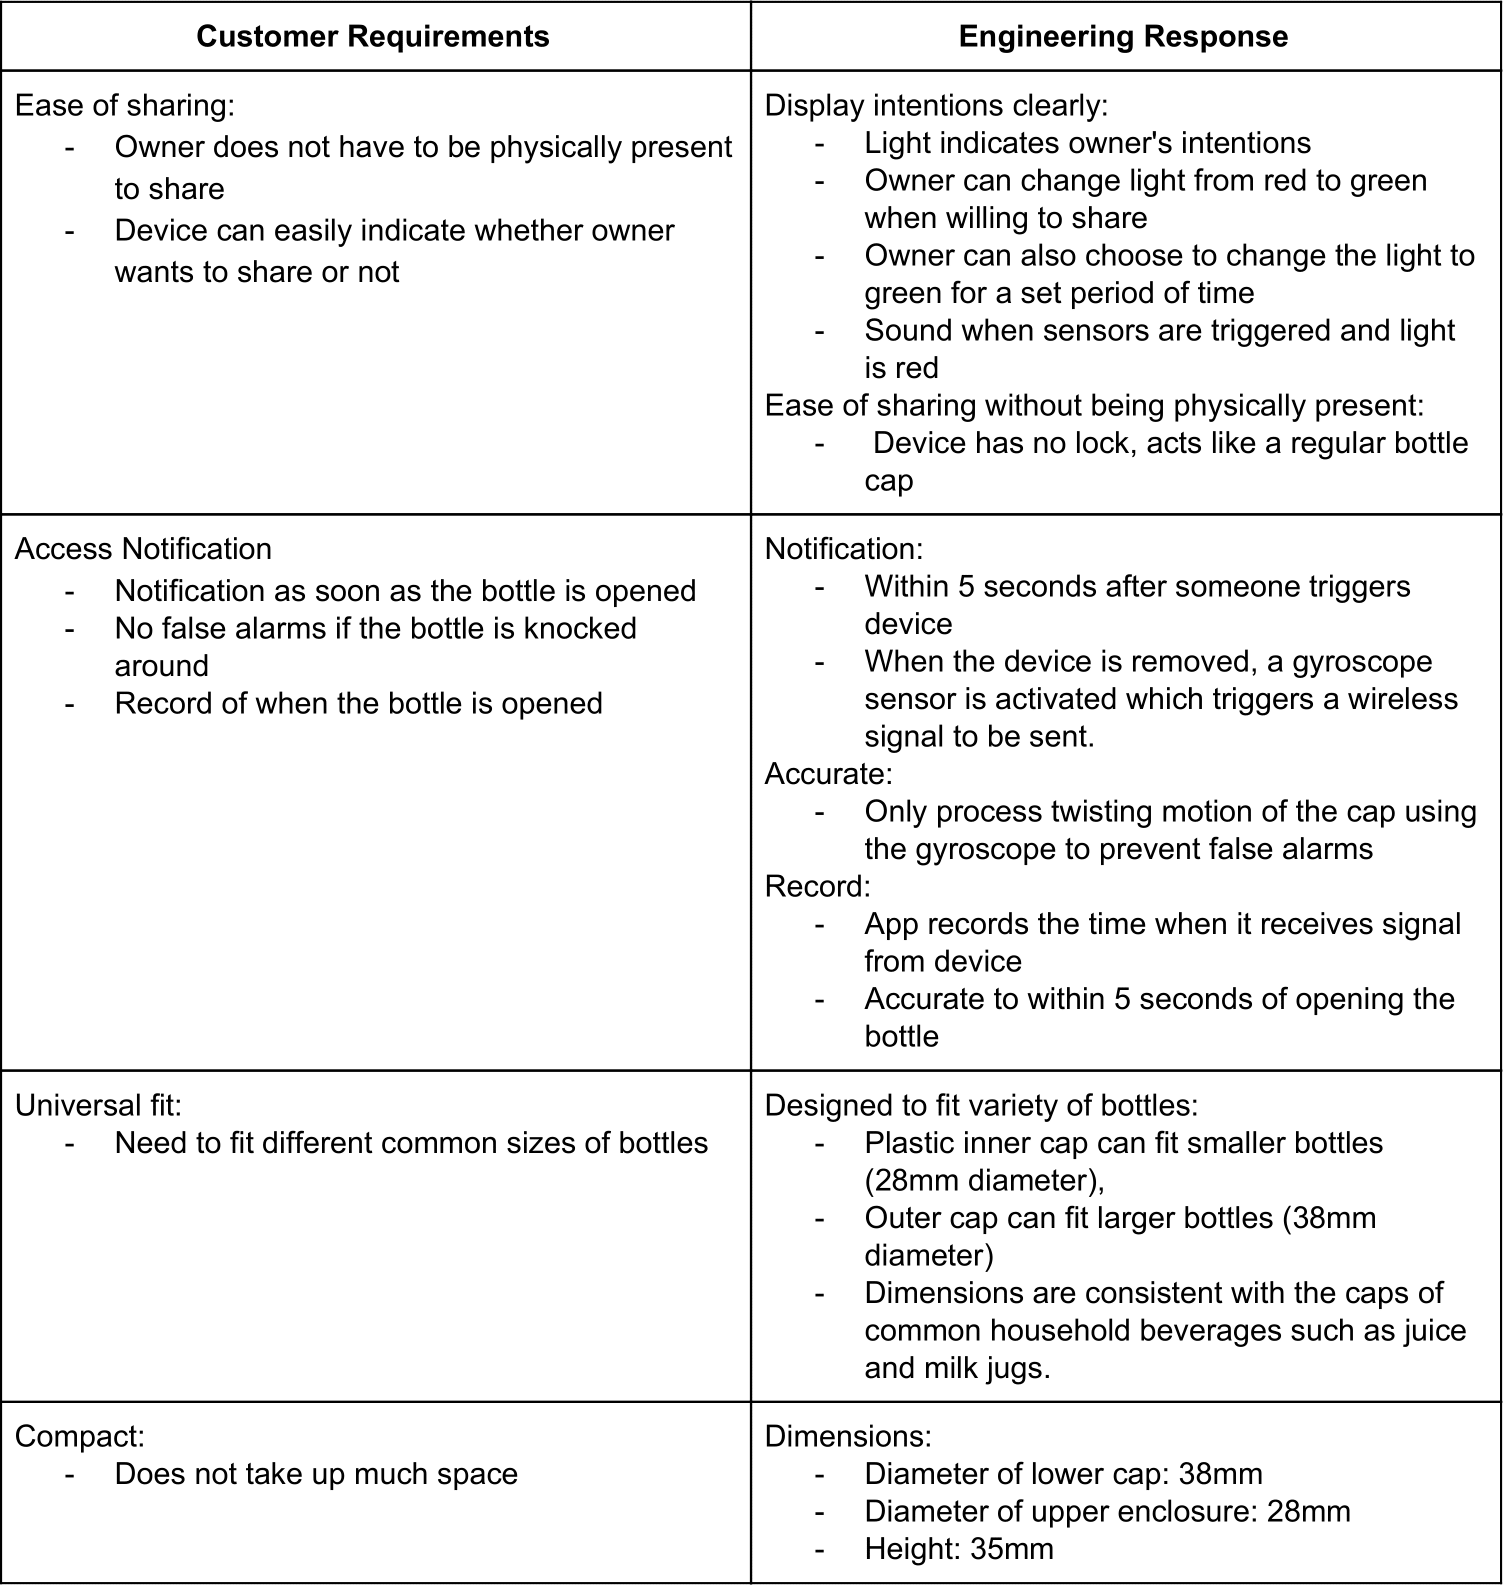
\includegraphics[width=\textwidth]{specs.png}
\end{figure}

		\addcontentsline{toc}{subsection}{Complete FMECA}
		\subsection*{Complete FMECA}

			\addcontentsline{toc}{subsection}{Detailed Bill of Materials}
	\subsection*{Detailed Bill of Materials}
	\begin{table}[H]
		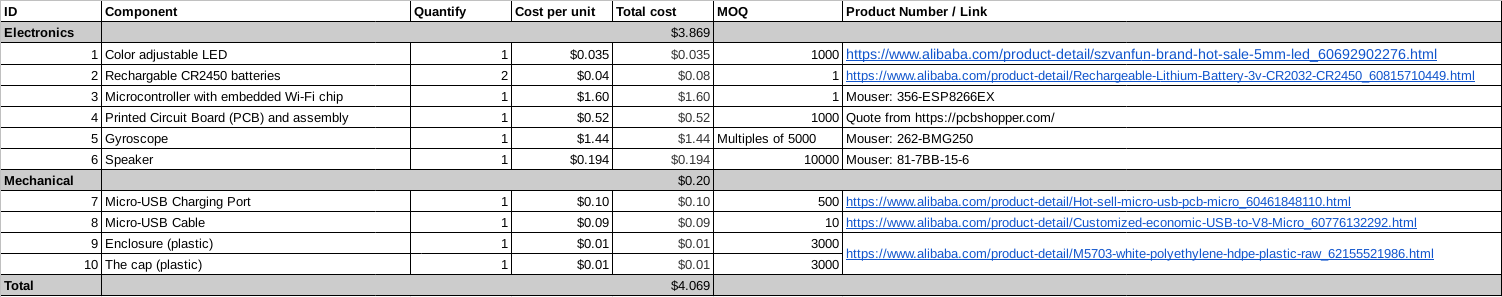
\includegraphics[width=\textwidth]{bom_large.png}
		
		\caption{Detailed BOM including product number or links to the source vendors. Mouser refers to Mouser.com.
		}
	\end{table}
			\subsection*{Detailed Work Breakdown Structure}
	\begin{table}[H]
		\centering
		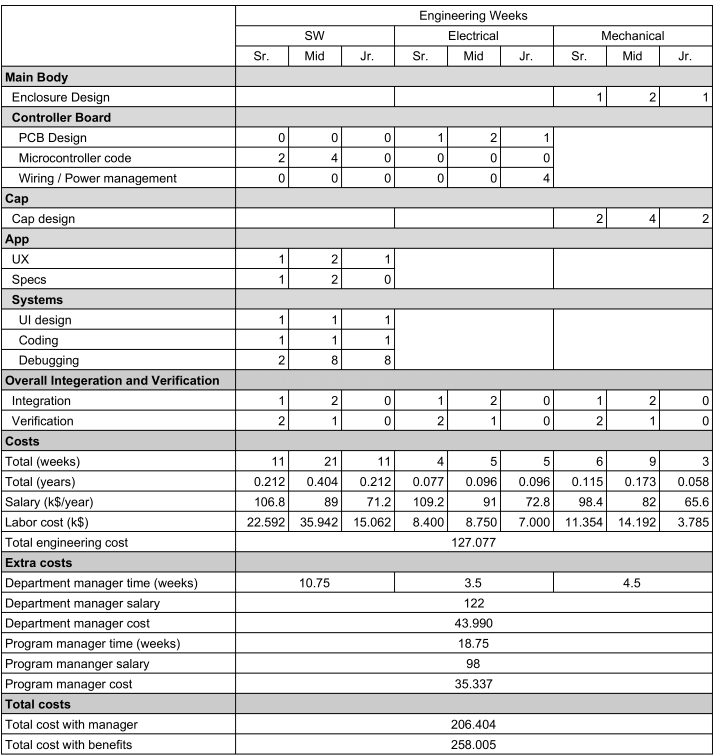
\includegraphics[width=\textwidth]{wbs_large3.png}
		\caption{ Detailed WBS including all detailed salary calculations and manager hours}
	\end{table}
		\addcontentsline{toc}{subsection}{Break Even Calculations}
		\subsection*{Break Even Calculations}
				\begin{table}[H]
			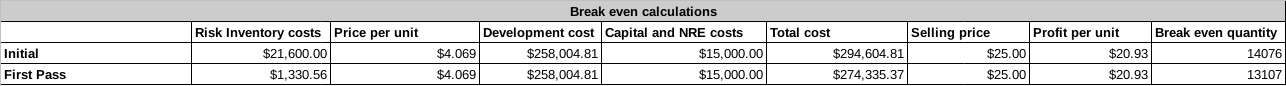
\includegraphics[width=\textwidth]{breakeven.png}
			
			\caption{ Break even calculations including initial and first pass
}
		\end{table}
		\addcontentsline{toc}{subsection}{Risk Inventory Calculations}
		\subsection*{Risk Inventory Calculations}
				\begin{table}[H]
			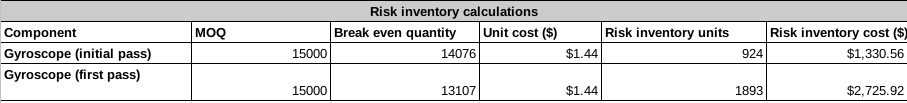
\includegraphics[width=\textwidth]{risk.png}
			\caption{Detailed risk inventory calculations}
		\end{table}
		
				\addcontentsline{toc}{subsection}{Detailed Work Breakdown Structure}

\end{document}